\documentclass{standalone}
\usepackage{tikz}
\usetikzlibrary{patterns, positioning}


\begin{document}
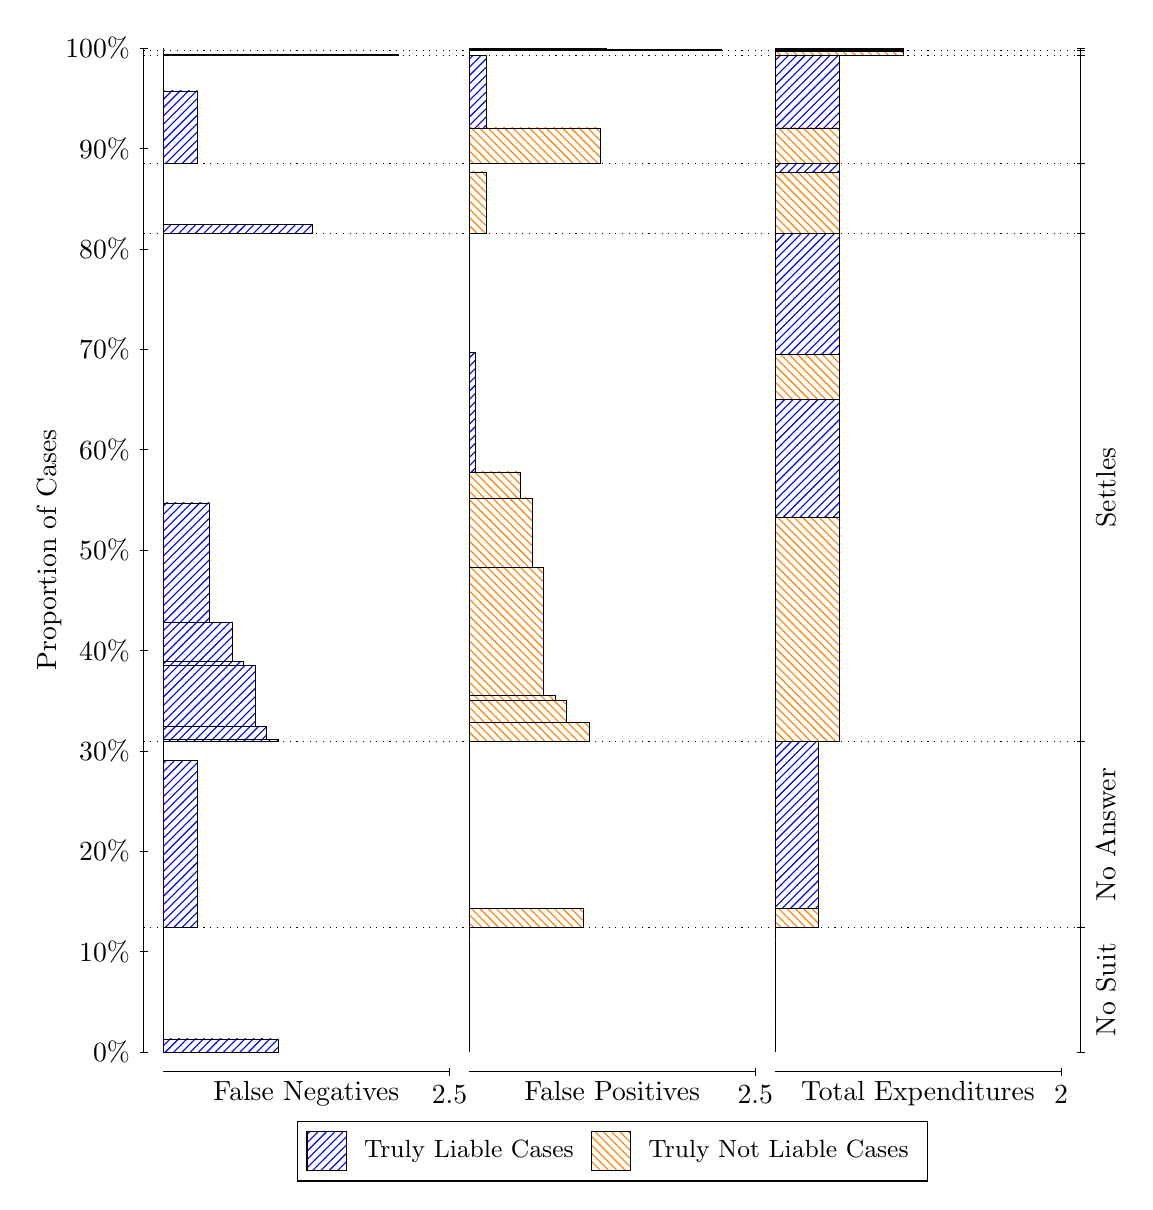
\begin{tikzpicture}
\draw[black, very thin] (1.5,1.75) -- (1.5,14.5);
\node[rotate=90, text=black, anchor=center] at (0.3, 8.125) {Proportion of Cases};
\draw[black, very thin] (1.45,1.75) -- (1.55,1.75);
\node[text=black, anchor=east] at (1.45, 1.75) {0\%};
\draw[black, very thin] (1.45,3.025) -- (1.55,3.025);
\node[text=black, anchor=east] at (1.45, 3.025) {10\%};
\draw[black, very thin] (1.45,4.3) -- (1.55,4.3);
\node[text=black, anchor=east] at (1.45, 4.3) {20\%};
\draw[black, very thin] (1.45,5.575) -- (1.55,5.575);
\node[text=black, anchor=east] at (1.45, 5.575) {30\%};
\draw[black, very thin] (1.45,6.85) -- (1.55,6.85);
\node[text=black, anchor=east] at (1.45, 6.85) {40\%};
\draw[black, very thin] (1.45,8.125) -- (1.55,8.125);
\node[text=black, anchor=east] at (1.45, 8.125) {50\%};
\draw[black, very thin] (1.45,9.4) -- (1.55,9.4);
\node[text=black, anchor=east] at (1.45, 9.4) {60\%};
\draw[black, very thin] (1.45,10.675) -- (1.55,10.675);
\node[text=black, anchor=east] at (1.45, 10.675) {70\%};
\draw[black, very thin] (1.45,11.95) -- (1.55,11.95);
\node[text=black, anchor=east] at (1.45, 11.95) {80\%};
\draw[black, very thin] (1.45,13.225) -- (1.55,13.225);
\node[text=black, anchor=east] at (1.45, 13.225) {90\%};
\draw[black, very thin] (1.45,14.5) -- (1.55,14.5);
\node[text=black, anchor=east] at (1.45, 14.5) {100\%};

\draw[black, very thin] (13.4,1.75) -- (13.4,14.5);
\draw[black, very thin] (13.35,1.75) -- (13.45,1.75);
\node[anchor=west] at (13.35, 1.75) {};
\draw[black, very thin] (13.35,3.3316) -- (13.45,3.3316);
\node[anchor=west] at (13.35, 3.3316) {};
\draw[black, very thin] (13.35,5.6924) -- (13.45,5.6924);
\node[anchor=west] at (13.35, 5.6924) {};
\draw[black, very thin] (13.35,12.148) -- (13.45,12.148);
\node[anchor=west] at (13.35, 12.148) {};
\draw[black, very thin] (13.35,13.035) -- (13.45,13.035);
\node[anchor=west] at (13.35, 13.035) {};
\draw[black, very thin] (13.35,14.409) -- (13.45,14.409);
\node[anchor=west] at (13.35, 14.409) {};
\draw[black, very thin] (13.35,14.469) -- (13.45,14.469);
\node[anchor=west] at (13.35, 14.469) {};
\draw[black, very thin] (13.35,14.5) -- (13.45,14.5);
\node[anchor=west] at (13.35, 14.5) {};

\draw[black, very thin, pattern color=blue, pattern=north east lines] (1.75,1.75) rectangle (3.2033,1.9164);
\draw[black, very thin, pattern color=orange, pattern=north west lines] (1.75,1.9164) rectangle (1.75,3.3316);
\draw[black, very thin, pattern color=blue, pattern=north east lines] (1.75,3.3316) rectangle (2.186,5.4485);
\draw[black, very thin, pattern color=orange, pattern=north west lines] (1.75,5.4485) rectangle (1.75,5.6924);
\draw[black, very thin, pattern color=blue, pattern=north east lines] (1.75,5.6924) rectangle (3.2033,5.7201);
\draw[black, very thin, pattern color=blue, pattern=north east lines] (1.75,5.7201) rectangle (3.058,5.8811);
\draw[black, very thin, pattern color=blue, pattern=north east lines] (1.75,5.8811) rectangle (2.9127,6.6589);
\draw[black, very thin, pattern color=blue, pattern=north east lines] (1.75,6.6589) rectangle (2.7673,6.7069);
\draw[black, very thin, pattern color=blue, pattern=north east lines] (1.75,6.7069) rectangle (2.622,7.2077);
\draw[black, very thin, pattern color=blue, pattern=north east lines] (1.75,7.2077) rectangle (2.3313,8.7226);
\draw[black, very thin, pattern color=orange, pattern=north west lines] (1.75,8.7226) rectangle (1.75,12.148);
\draw[black, very thin, pattern color=blue, pattern=north east lines] (1.75,12.148) rectangle (3.6393,12.257);
\draw[black, very thin, pattern color=orange, pattern=north west lines] (1.75,12.257) rectangle (1.75,13.035);
\draw[black, very thin, pattern color=blue, pattern=north east lines] (1.75,13.035) rectangle (2.186,13.957);
\draw[black, very thin, pattern color=orange, pattern=north west lines] (1.75,13.957) rectangle (1.75,14.409);
\draw[black, very thin, pattern color=blue, pattern=north east lines] (1.75,14.409) rectangle (4.7293,14.424);
\draw[black, very thin, pattern color=orange, pattern=north west lines] (1.75,14.424) rectangle (1.75,14.469);
\draw[black, very thin, pattern color=orange, pattern=north west lines] (1.75,14.469) rectangle (1.75,14.484);
\draw[black, very thin, pattern color=blue, pattern=north east lines] (1.75,14.484) rectangle (1.75,14.5);
\draw[black, very thin, pattern color=orange, pattern=north west lines] (5.6333,1.75) rectangle (5.6333,3.1652);
\draw[black, very thin, pattern color=blue, pattern=north east lines] (5.6333,3.1652) rectangle (5.6333,3.3316);
\draw[black, very thin, pattern color=orange, pattern=north west lines] (5.6333,3.3316) rectangle (7.0867,3.5755);
\draw[black, very thin, pattern color=blue, pattern=north east lines] (5.6333,3.5755) rectangle (5.6333,5.6924);
\draw[black, very thin, pattern color=orange, pattern=north west lines] (5.6333,5.6924) rectangle (7.1593,5.9337);
\draw[black, very thin, pattern color=orange, pattern=north west lines] (5.6333,5.9337) rectangle (6.8687,6.2147);
\draw[black, very thin, pattern color=orange, pattern=north west lines] (5.6333,6.2147) rectangle (6.7233,6.2744);
\draw[black, very thin, pattern color=orange, pattern=north west lines] (5.6333,6.2744) rectangle (6.578,7.9001);
\draw[black, very thin, pattern color=orange, pattern=north west lines] (5.6333,7.9001) rectangle (6.4327,8.7875);
\draw[black, very thin, pattern color=orange, pattern=north west lines] (5.6333,8.7875) rectangle (6.2873,9.1179);
\draw[black, very thin, pattern color=blue, pattern=north east lines] (5.6333,9.1179) rectangle (5.706,10.633);
\draw[black, very thin, pattern color=blue, pattern=north east lines] (5.6333,10.633) rectangle (5.6333,12.148);
\draw[black, very thin, pattern color=orange, pattern=north west lines] (5.6333,12.148) rectangle (5.8513,12.926);
\draw[black, very thin, pattern color=blue, pattern=north east lines] (5.6333,12.926) rectangle (5.6333,13.035);
\draw[black, very thin, pattern color=orange, pattern=north west lines] (5.6333,13.035) rectangle (7.3047,13.487);
\draw[black, very thin, pattern color=blue, pattern=north east lines] (5.6333,13.487) rectangle (5.8513,14.409);
\draw[black, very thin, pattern color=orange, pattern=north west lines] (5.6333,14.409) rectangle (5.6333,14.454);
\draw[black, very thin, pattern color=blue, pattern=north east lines] (5.6333,14.454) rectangle (5.6333,14.469);
\draw[black, very thin, pattern color=orange, pattern=north west lines] (5.6333,14.469) rectangle (8.8307,14.484);
\draw[black, very thin, pattern color=blue, pattern=north east lines] (5.6333,14.484) rectangle (7.3773,14.5);
\draw[black, very thin, pattern color=orange, pattern=north west lines] (9.5167,1.75) rectangle (9.5167,3.1652);
\draw[black, very thin, pattern color=blue, pattern=north east lines] (9.5167,3.1652) rectangle (9.5167,3.3316);
\draw[black, very thin, pattern color=orange, pattern=north west lines] (9.5167,3.3316) rectangle (10.062,3.5755);
\draw[black, very thin, pattern color=blue, pattern=north east lines] (9.5167,3.5755) rectangle (10.062,5.6924);
\draw[black, very thin, pattern color=orange, pattern=north west lines] (9.5167,5.6924) rectangle (10.334,8.5462);
\draw[black, very thin, pattern color=blue, pattern=north east lines] (9.5167,8.5462) rectangle (10.334,10.034);
\draw[black, very thin, pattern color=orange, pattern=north west lines] (9.5167,10.034) rectangle (10.334,10.606);
\draw[black, very thin, pattern color=blue, pattern=north east lines] (9.5167,10.606) rectangle (10.334,12.148);
\draw[black, very thin, pattern color=orange, pattern=north west lines] (9.5167,12.148) rectangle (10.334,12.926);
\draw[black, very thin, pattern color=blue, pattern=north east lines] (9.5167,12.926) rectangle (10.334,13.035);
\draw[black, very thin, pattern color=orange, pattern=north west lines] (9.5167,13.035) rectangle (10.334,13.487);
\draw[black, very thin, pattern color=blue, pattern=north east lines] (9.5167,13.487) rectangle (10.334,14.409);
\draw[black, very thin, pattern color=orange, pattern=north west lines] (9.5167,14.409) rectangle (11.152,14.454);
\draw[black, very thin, pattern color=blue, pattern=north east lines] (9.5167,14.454) rectangle (11.152,14.469);
\draw[black, very thin, pattern color=orange, pattern=north west lines] (9.5167,14.469) rectangle (11.152,14.484);
\draw[black, very thin, pattern color=blue, pattern=north east lines] (9.5167,14.484) rectangle (11.152,14.5);
\draw[black, dotted] (1.5,3.3316) -- (13.4,3.3316);
\draw[black, dotted] (1.5,5.6924) -- (13.4,5.6924);
\draw[black, dotted] (1.5,12.148) -- (13.4,12.148);
\draw[black, dotted] (1.5,13.035) -- (13.4,13.035);
\draw[black, dotted] (1.5,14.409) -- (13.4,14.409);
\draw[black, dotted] (1.5,14.469) -- (13.4,14.469);
\draw[black, very thin] (1.75,1.5) -- (5.3833,1.5);
\node[text=black, anchor=north] at (3.5667, 1.5) {False Negatives};
\draw[black, very thin] (5.3833,1.45) -- (5.3833,1.55);
\node[text=black, anchor=north] at (5.3833, 1.45) {2.5};

\draw[black, very thin] (5.6333,1.5) -- (9.2667,1.5);
\node[text=black, anchor=north] at (7.45, 1.5) {False Positives};
\draw[black, very thin] (9.2667,1.45) -- (9.2667,1.55);
\node[text=black, anchor=north] at (9.2667, 1.45) {2.5};

\draw[black, very thin] (9.5167,1.5) -- (13.15,1.5);
\node[text=black, anchor=north] at (11.333, 1.5) {Total Expenditures};
\draw[black, very thin] (13.15,1.45) -- (13.15,1.55);
\node[text=black, anchor=north] at (13.15, 1.45) {2};

\node[text=black, centered, rotate=90] at (13.72, 2.5408) {No Suit};
\node[text=black, centered, rotate=90] at (13.72, 4.512) {No Answer};
\node[text=black, centered, rotate=90] at (13.72, 8.9202) {Settles};





\draw (7.449999999999999,1.5) node[draw=none] (baseCoordinate) {};
\begin{scope}[align=center]
        \matrix[scale=0.5, draw=black, below=0.5cm of baseCoordinate, nodes={draw}, column sep=0.1cm]{
            \node[rectangle, draw, minimum width=0.5cm, minimum height=0.5cm, pattern color=blue, pattern=north east lines] {}; &
            \node[draw=none, font=\small, text=black] (B) {Truly Liable Cases}; &
            \node[rectangle, draw, minimum width=0.5cm, minimum height=0.5cm, pattern color=orange, pattern=north west lines] {}; &
            \node[draw=none, font=\small, text=black] (B) {Truly Not Liable Cases}; \\
            };
\end{scope}

\end{tikzpicture}
\end{document}